\documentclass[11pt, oneside]{article}   	
\usepackage{geometry}                		
\geometry{letterpaper}                   		
\usepackage{graphicx}				
\usepackage{amssymb}

\title{Compiler Construction/Fall 2014/Homework 1}
\author{Abhi Agarwal}
\date{}							

\begin{document}
\maketitle

\section{Language Processors}
\subsection{Question 1.1}
\par The front-end of a compiler deals with the language itself, and the back-end of a compiler deals with code generation for a specific computer. 
\par The reason we would want to separate them is to improve portability. If you've to different computers you can use the same front-end, but write different back-ends for them. This is because of the fact that we don't have to generate any machine-specific code when doing semantic analysis, or IR generation, or in any of the steps in the front-end - we can use the same codebase from this section in all computers. However, for the backend the process of generating machine dependent code changes from computer to computer. Different computers use different builds, and so we've to create different backends to process the IR from the front-end and make it into machine code. So it allows us to reuse some of our codebase again, it helps in convenience for the compiler team, and to keep things standardized between different backends.
\par Some teams have also situations where they use the same back-end with different front-ends. If you're creating a new language you mostly only need to rewrite or tweak your front-end as this is how the language is defined, and so the back-end stays the same. If individuals are in the field of consulting in creating Domain Specific Languages they can rewrite parts of the front-end and use the same back-end system. This is of course if they are writing it for one system - or if they already have the backend written for the different systems.
\par Also I think it's a good practice to separate these things. You can write tests for different parts of the system, and you can almost guarantee that the front-end should work globally on all computers. You can also write tests for individual computers, and see if that works.

\newpage

\subsection{Question 1.2}
\par From the notes it suggests that there's usually an optimizer after/at the intermediary representation generator level or IR level, and after/at the machine dependent code generation level. This suggest that there is one in-between the front-end and the back-end, and one before the compiler outputs a target program.
\par Lets assume we have generated some front-end code, and now we want to use it with some back-end system. We would optimize it so that it can be plugged into any different back-end system, and behave the same way. When we generate some output from the front-end system we can take that input and use it with different back-end parts because it hasn't been compiled into machine-specific code. Therefore, we can optimize as a way to standardize all the front-end generated code so it can be put into any back-end part, and so any different computer.

\section{Compiler Phases}
\subsection{Question 2.1}
\par \small $<$id, 1$>$ $<$=$>$ $<$($>$ $<$id, 2$>$ $<$-$>$ $<$num, 32$>$ $<$)$>$ $<$*$>$ $<$($>$ $<$num, 5$>$ $<$/$>$ $<$num, 9$>$ $<$)$>$
\par where the symbol table is as follows: 
\par \begin{tabular}{ l | c }
  1  & celsius \\
  2 & fahrenheit \\
\end{tabular}

\subsection{Question 2.2}
\par Drawing the tree for the syntax above. It is parsed into a syntax tree. Here we some-what decide if the syntax can not be parsed.

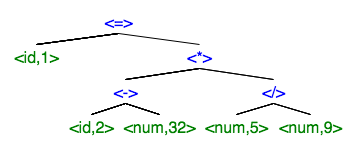
\includegraphics[]{image1.png}

\newpage

\subsection{Question 2.3}
\par Converting using the int2float function. It is enriched with semantic information.

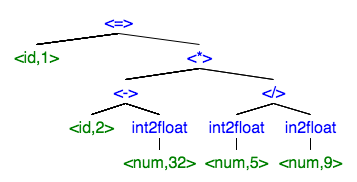
\includegraphics[]{image2.png}

\subsection{Question 2.4}
\par We translate it into intermediate code. Some of this is what we did in class so I'm using the steps and terminology used in class.
\par t1 = inttofloat(32)
\par t2 = fahrenheit - t1
\par t3 = inttofloat(5)
\par t4 = inttofloat(9)
\par t5 = t3/t5
\par t6 = t2 * t5
\par id1 = t6

\subsection{Question 2.5}
\par Then there is optimization to code. This process was somewhat given by example in class as well.
\par t1 = id2 - 32.0 \par id1 = t1 *  0.556
\par Basically id2 is referencing fahrenheit (I think this is how you use things from symbol table?), and conversion from $(5/6)$ to 0.55556, but I left it in short form.

\newpage

\subsection{Question 2.6}
\par I'm taking some inspiration from the notes for this question. I'm going to be moving the ID2 into the R2 register, then subtracting it with 32.0, and then multiplying it with 0.556, and then loading it back into ID1, which is some memory address we have. So here we have 2 memory addresses that I'm assuming I've stored somewhere: ID1, ID2, and they just load a parameter, and then store it into celsius where the user gets his/her answer.
\par LDF R2, ID2
\par SUBF R2, 32.0
\par MULF R2, 0.556
\par LDF ID1, R2

\section{Programming}
\subsection{Question 3.1}
\par Each language has a specification document. How is the grammar described for each language? How is the meaning of each programming construct described for the language?
\par Compiled languages examples: C, C++, Objective-C, Go, Haskell, Visual Basic, Ada.
\par Interpreted languages examples: R, S, Ruby, Python, PHP, Matlab, Javascript.

\end{document}  